\section[Paper VI: A multi-modal sleep event detection model for clinical sleep analysis]{Paper VI: A multi-modal sleep event detection model for clinical sleep analysis%
    \sectionmark{Olesen, Jennum, Mignot, \& Sorensen, 2020c \textit{(in preparation)}}}\label{sec:papervi}
\sectionmark{Olesen, Jennum, Mignot, \& Sorensen, 2020c \textit{(in preparation)}}

\begin{tcolorbox}[colframe=white]
\paragraph{Study objective: } Clinical sleep analysis require manual analysis of sleep patterns for correct diagnosis of sleep disorders.
Several studies show significant variability in scoring discrete sleep events.
We wished to investigate, whether an automatic method could be used for detection of arousals (Ar), leg movements (LM) and sleep disordered breathing (SDB) events, and if the joint detection of these events performed better than having three separate models.
\paragraph{Methods: } We designed a single deep neural network architecture to jointly detect sleep events in a polysomnogram.
We trained the model on 1653 recordings of individuals, and tested the optimized model on 1000 separate recordings. 
The performance of the model was quantified by F1, precision, and recall scores, and by correlating index values to clinical values using Pearson's correlation coefficient.
\paragraph{Results: } F1 scores for the optimized model was 0.70, 0.63, and 0.62 for Ar, LM, and SDB, respectively. 
The performance was higher, when detecting events jointly compared to corresponding single-event models.
Index values computed from detected events correlated well with manual annotations (\(r^2 = 0.73, \, r^2 = 0.77, \, r^2 = 0.78\), respectively).
\paragraph{Conclusion: } Detecting arousals, leg movements and sleep disordered breathing events jointly is possible, and the computed index values correlates well with human annotations.
\end{tcolorbox}

Clinical sleep analysis is currently performed manually by experts based on guidelines from the \ac{AASM} detailed in the \ac{AASM} Scoring Manual~\cite{Berry2020}.
The guidelines detail both technical and clinical best practices for setting up and recording \acp{PSG}, which are overnight recordings of various electrophysiological signals, such as \ac{EEG}, \ac{EOG}, chin and leg \ac{EMG}, \ac{ECG}, respiratory inductance plethysmography from the thorax and abdomen, oronasal pressure, and blood oxygen levels.

Based on these signals, expert technicians analyse and score the \ac{PSG} for sleep stages [\ac{W}, \ac{REM} sleep, \ac{N1}, \ac{N2}, and \ac{N3}], and sleep micro-events summarized in key metrics, such as the \ac{AHI} (number of apneas and hypopneas per hour of sleep), the \ac{PLMI} (number of period leg movements per hour of sleep), and the \ac{ArI} (number of arousals per hour of sleep).

Arousals are defined as abrupt shifts in \ac{EEG} frequencies towards alpha, theta, and beta rhythms for at least \SI{3}{\second} with a preceding period of stable sleep of at least \SI{10}{\second}.
During \ac{REM} sleep, where the background \ac{EEG} shows similar rhythms, arousal scoring requires a concurrent increase in chin \ac{EMG} lasting at least \SI{1}{\second}.
\Acp{LM} should be scored in the leg \ac{EMG} channels, when there is an increase in amplitude of at least \SI{8}{\micro\volt} above baseline level with a duration between \SIrange{0.5}{10}{\second}.
A \ac{PLM} series is then defined as a sequence of 4 \acp{LM}, where the time between \ac{LM} onsets is between \SIrange{5}{90}{\minute}.
Apneas are generally scored when there is a complete (\SI{>=90}{\percent} of pre-event baseline) cessation of breathing activity either due to a physical obstruction (obstructive apnea) or due to an underlying disruption in the central nervous system control (central apnea) for at least \SI{10}{\second}.
When the breathing is only partially reduced (\SI{>=30}{\percent} of pre-event baseline) and the duration of the excursion is \SI{>=10}{\second}, the event is scored as a hypopnea if there is either a \SI{>=4}{\percent} oxygen desaturation or a \SI{>=3}{\percent} oxygen desaturation coupled with an \ac{Ar}.

However, several studies have shown significant variability in the scoring of both sleep stages~\cite{Norman2000, Danker-Hopfe2004, Danker-Hopfe2009, Rosenberg2013, Zhang2015a, Younes2016, Younes2018} and sleep micro-events~\cite{Drinnan1998, Whitney1998, Loredo1999, Smurra2001, Thomas2003, Bonnet2007, Magalang2013, Rosenberg2014}.
This has prompted extensive research into automatic methods for classifying sleep stages in large-scale studies~\cite{Koch2014, Supratak2017, Chambon2018c, Olesen2018c, Biswal2018, Stephansen2018, Phan2019a, Phan2019b}, while the research in automatic arousal~\cite{Olesen2019, Alvarez-Estevez2019, Brink-Kjaer2020} and \ac{LM}~\cite{Carvelli2020} detection on a similar scale is limited.
\citeauthor{Biswal2018} recently proposed a model based on a combination of recurrent and convolutional neural networks, where the same architecture was used for sleep stage classification, \ac{AHI} and \ac{LMI} prediction.
They trained their model using \num{9000} \ac{PSG} recordings and evaluated the performance on the three tasks on a held out test set containing \num{1000} \acp{PSG}. 
However, this model was trained in separate runs for each downstream task; furthermore, post-processing was performed on the event predictions (apneas, limb movements).

In this study, we introduce the \ac{MSED} model for joint detection of sleep micro-events, in this case \acp{Ar}, \ac{SDB}, and \acp{LM}.
The model is based on recent advances in machine learning and challenges current state of the art methods by directly classifying and localizing sleep micro-events in the \ac{PSG} signals at the same time.

\subsection{Data}

% \subsection{MrOS Sleep Study}
We collected \acp{PSG} from the MrOS Sleep Study, an ancillary part of the larger Osteoporotic Fractures in Men Study.
The main goal of the study is to research and discover connections between sleep disorders, skeletal fractures, and cardiovascular disease and mortality in community-dwelling older (\num{>65} years)~\cite{Blank2005,Orwoll2005,Blackwell2011}.
Of the original 5994 study participants, 3135 subjects were enrolled at one of six sites in the USA for a comprehensive sleep assessment, while 2909 of these underwent a full-night in-home \ac{PSG} recording,
The \ac{PSG} studies were subsequently scored by certified sleep technicians.
Sleep stages were scored into stages 1, 2, 3, 4 and \ac{REM}, while stages 3 and 4 combined into \ac{SWS} according to R\&K rules~\cite{Rechtschaffen1968}.
\acp{Ar} were scored as abrupt increases in \ac{EEG} frequencies lasting at least \SI{3}{\second} according to \ac{ASDA} rules~\cite{AmericanSleepDisordersAssociation1992}.
Apneas were defined as complete or near complete cessation of airflow lasting more than \SI{10}{\second} with an associated \SI{3}{\percent} or greater \ce{SaO2} desaturation, while hypopneas were based on a clear reduction in breathing of more than \SI{30}{\percent} deviation from baseline breathing lasting more than \SI{10}{\second}, and likewise assocated with a greater than \SI{3}{\percent} \ce{SaO2} desaturation.
While the scoring criteria for scoring \acp{LM} are not explicitly available for the MrOS Sleep Study, the prevailing standard at the time of the study was to score \acp{LM} following an increase in leg \ac{EMG} amplitude of more than \SI{8}{\micro\volt} above resting baseline levels for at least \SI{0.5}{\second}, but shorter than \SI{10}{\second}~\cite{Zucconi2006}.

\subsubsection{Subset demographics and partitioning}
We used a total of \num{2853} \ac{PSG} studies downloaded from the \ac{NSRR}~\cite{Dean2016,Zhang2018}, which we partitioned into a training set (\(\mathcal{D}_\textsc{train}\), \( n_{\text{train}} = 1653 \)), a validation set (\(\mathcal{D}_\textsc{eval}\), \(n_{\text{eval}} = 200\)), and a final testing set (\(\mathcal{D}_\textsc{test}\), \(n_{\text{test}} = 1000 \)).
Key demographics and \ac{PSG}-related variables for each subset are shown as mean \(\pm\) standard deviation with range in parenthesis in~\cref{tab:demographics}.

\begin{table*}[t]
    \small
    % \centering
    \renewcommand{\arraystretch}{1.2}
    \begin{adjustwidth*}{}{-\marginparwidth-\marginparsep}
    \begin{threeparttable}
        \caption{MrOS demographics by subset.}\label{tab:demographics}
        \begin{tabular}{@{}lcccc@{}}
        \toprule
        & \(\mathcal{D}_\textsc{train}\) & \(\mathcal{D}_\textsc{eval}\) & \(\mathcal{D}_\textsc{test}\) & \textit{p}-value \\
        \midrule
        \textit{n}                                  & 1653                          & 200                            & 1000                          & - \\
        Age, years                                  & \meanstdrange{76.4}{5.6}{67.0}{90.0}    & \meanstdrange{76.8}{5.4}{68.0}{90.0}     & \meanstdrange{76.4}{5.3}{67.0}{90.0}    & 0.404   \\
        \acs{BMI}, \si{\kilogram\per\square\second} & \meanstdrange{27.3}{3.9}{16.0}{47.0}    & \meanstdrange{27.0}{3.6}{19.0}{40.0}     & \meanstdrange{27.0}{3.7}{17.0}{45.0}    & 0.247   \\ \midrule
        \acs{TST}, \si{\minute}                     & \meanstdrange{357.3}{69.0}{54.0}{615.0} & \meanstdrange{354.0}{69.1}{108.0}{503.0} & \meanstdrange{353.6}{68.7}{62.0}{572.0} & 0.312   \\
        SL, \si{\minute}                      & \meanstdrange{22.9}{25.6}{1.0}{349.0}   & \meanstdrange{21.6}{23.0}{1.0}{135.0}    & \meanstdrange{25.1}{32.1}{1.0}{402.0}   & 0.284   \\
        \acs{REML}, \si{\minute}                    & \meanstdrange{109.5}{77.9}{0.0}{578.0}  & \meanstdrange{103.5}{70.0}{10.0}{413.0}  & \meanstdrange{107.2}{75.3}{3.0}{590.0}  & 0.466   \\
        \acs{WASO}, \si{\minute}                    & \meanstdrange{116.7}{67.1}{11.0}{462.0} & \meanstdrange{119.0}{70.8}{15.0}{372.0}  & \meanstdrange{112.9}{65.0}{6.0}{458.0}  & 0.471   \\
        SE, \si{\percent}                     & \meanstdrange{75.9}{12.1}{17.0}{97.0}   & \meanstdrange{75.5}{12.3}{37.0}{96.0}    & \meanstdrange{76.4}{11.8}{26.0}{98.0}   & 0.690    \\
        \acs{N1}, \si{\percent}                     & \meanstdrange{6.8}{4.1}{0.0}{31.0}      & \meanstdrange{7.0}{4.5}{0.0}{28.0}       & \meanstdrange{6.9}{4.7}{1.0}{58.0}      & 0.968   \\
        \acs{N2}, \si{\percent}                     & \meanstdrange{62.7}{9.5}{28.0}{89.0}    & \meanstdrange{62.0}{9.7}{30.0}{90.0}     & \meanstdrange{62.8}{10.0}{21.0}{95.0}   & 0.451   \\
        \acs{N3}, \si{\percent}                     & \meanstdrange{11.4}{9.0}{0.0}{55.0} 	& \meanstdrange{11.8}{9.7}{0.0}{55.0} 	 & \meanstdrange{11.1}{9.0}{0.0}{57.0}     & 0.638 \\
        \acs{REM}, \si{\percent}                    & \meanstdrange{19.2}{6.5}{0.0}{44.0}     & \meanstdrange{19.4}{7.2}{0.0}{41.0}      & \meanstdrange{19.3}{6.7}{0.0}{42.0}     & 0.894   \\ \midrule
        \acs{ArI}, \si{\per\hour}                   & \meanstdrange{23.5}{11.8}{3.0}{87.0}    & \meanstdrange{23.4}{11.0}{4.0}{77.0}     & \meanstdrange{23.8}{11.8}{4.0}{102.0}   & 0.661   \\
        \acs{AHI}, \si{\per\hour}                   & \meanstdrange{13.5}{13.9}{0.0}{83.0}    & \meanstdrange{13.6}{13.3}{0.0}{59.0}     & \meanstdrange{14.2}{15.5}{0.0}{89.0}    & 0.907   \\
        \acs{PLMI}, \si{\per\hour}                  & \meanstdrange{35.4}{37.1}{0.0}{233.0}   & \meanstdrange{36.6}{39.0}{0.0}{178.0}    & \meanstdrange{36.0}{37.7}{0.0}{175.0}   & 0.993   \\ \bottomrule
        \end{tabular}
        \begin{tablenotes}
            \item Data are shown as means \(\pm\) standard deviations (range) across \acp{PSG}. Variables were tested with Kruskal-Wallis \textit{H}-tests. Significant \textit{p}-values at significance level \( \alpha = 0.05 \) are highlighted in bold. %
            \describe{BMI}; %
            \describe{TST}; %
            SL, sleep latency, %
            % \describe{SL}; %
            \describe{REML}; %
            \describe{WASO}; %
            SE, sleep efficiency, %
            % \describe{SE}; %
            \describe{N1}; %
            \describe{N2}; %
            \describe{N3}; %
            \describe{REM}; %
            \describe{ArI}; %
            \describe{AHI}; %
            \describe{PLMI}.
        \end{tablenotes}
    \end{threeparttable}
    \end{adjustwidth*}
\end{table*}


\subsubsection{Signal and events}
For this study, we considered three \ac{PSG} events: \acp{Ar}, \acp{LM}, and \ac{SDB} events, which includes all forms of apneas (obstructive and central) and hypopneas.
These event types are each based on a specific set of electrophysiological channels from the \ac{PSG}, and as such, we extracted left and right central \ac{EEG} (C3 and C4), left and right \ac{EOG}, left and right chin \ac{EMG}, left and right leg \ac{EMG}, nasal pressure, and respiratory inductance plethysmography from the thorax and abdomen.
\Ac{EEG} and \ac{EOG} channels were referenced to the contralateral mastoid process, while a chin \ac{EMG} was synthesized by subtracting the right chin \ac{EMG} from the left chin \ac{EMG}.

Apart from the raw signal data, we also extracted onset time relative to the study start time and duration times for each event type in each \ac{PSG}.

% In this study, we only considered the detection of two PSG events, arousals and leg movements. These events are characterized by a start time and a duration, which we extracted from 2,907 PSG studies from visit 1 available from the National Sleep Research Resource repository~\cite{Dean2016,Zhang2018}. From each PSG study, we extracted left and right central EEG, left and right EOG, chin EMG, and EMG from the left and right anterior tibialis. EEG and EOG channels were referenced to the contralateral mastoid process, while a leg EMG channel was synthesized by referencing left to right. Any PSG without the full set of channels or without any event scoring was eliminated from further analysis.


\subsection{Methods}

\paragraph{Notation}
We denote by \(\llbracket a, b \rrbracket\) the set of integers \(\lbrace n \in \N \mid a \leq n \leq b\rbrace\) with \(\llbracket N \rrbracket\) being shorthand for \(\llbracket 1, N \rrbracket\), and by \(n \in \llbracket N \rrbracket \) the \textit{n}th sample in \(\llbracket N \rrbracket\).
A segment of PSG data is denoted by \(\mathbf{x} \in \R{C \times T}\), where \(C, T\) is the number of channels and the duration of the segment in samples, respectively.
The corresponding set of \(N_t\) true events for the segment is denoted by \( \boldsymbol{\varepsilon}^{t} = \braces*{ \parentheses*{ \varrho^{t}_{i}, \delta^{t}_{i}} \in \R{2}_+ \mid i \in \bbrackets*{ N_{t} } } \), where \(\varrho, \delta\) are the center point and duration, respectively, of the \textit{i}th event.
By \(\mathbf{\chi} \in \mathcal{D}_\ast\) we denote a sample in either one of the three subsets.
In the description of the network architecture, we have omitted the batch dimension from all calculations for brevity.

\subsubsection{Model overview}

Given an input set \( \boldsymbol{\chi} = \braces*{\mathbf{x}, \boldsymbol{\varepsilon}^t} \in \R{C \times T} \times \R{N_t \times 2}_+ \) containing \ac{PSG} data with \(C\) channels and \(T\) time steps, and true events \(\boldsymbol{\varepsilon}\), the goal of the model is to detect any possible events in the segment, where, in this context, detection covers both classification \textit{and} localization of any event in the segment space.

To accomplish this, the model generates a set of \textit{default event windows} \(\boldsymbol{\varepsilon}^d = \braces*{ \parentheses*{ \varrho^{d}_j, \delta^d_j } \in \R{2}_+ \mid j \in \bbrackets*{N_d} }\) for the current segment, and match each true event to a default event window if their intersection-over-union (IoU) is at least 0.5.

At test time, we generate predictions over the default event windows and use a non-maximum suppression procedure to select between the candidate predictions.
For a given class \textit{k}, the procedure is as follows.
First, the predictions are sorted according to probability of the event, which is above a threshold \(\theta_k\).
Then, using the most probable prediction as an anchor, we sequentially evaluate the IoU between the anchor and the remaining candidate predictions, removing those with \(\text{IoU}>=0.5\).

The output of the model is thus the set \(\braces*{\mathbf{p}, \mathbf{y}}\) containing the predicted class probabilities along with the corresponding onsets and durations.


% Given an input tensor set \( \boldsymbol{\chi} = \braces*{\mathbf{x}, \boldsymbol{\pi}, \mathbf{t}} \in \R{C \times T} \times \R{N_m \times \hat{K}} \times \R{N_m \times 2} \) containing \ac{PSG} data with \(C\) channels and \(T\) time steps, the one-hot encoded target class labels in \( \boldsymbol{\pi} \), and the encoded, matched target event onsets and durations in \( \mathbf{t} \), the goal of the model is to detect any possible events in the segment.
% In this context, detection covers both classification \textit{and} localization of any event.
% To do this, we generate a set of \textit{default event windows} \(\boldsymbol{\varepsilon}^d = \braces*{ \parentheses*{ \varrho^{d}_j, \delta^d_j } \in \R{2}_+ \mid j \in \bbrackets*{N_d} }\)

% The input data segment to the network is a tensor set \( \boldsymbol{\chi} = \braces*{\mathbf{x}, \boldsymbol{\pi}, \mathbf{t}} \in \R{C \times T} \times \R{N_m \times \hat{K}} \times \R{N_m \times 2} \) containing \ac{PSG} data with \(C\) channels and \(T\) time steps, the one-hot encoded target class labels in \( \boldsymbol{\pi} \), and the encoded target event onset and duration in \( \mathbf{t} \) for the \( N_m \in \mathbb{N} \) default event windows in the data segment, that is matched to true events.

% We used a bipartite matching sheme

\subsubsection{Signal processing pipeline}
We resampled all signals to a common sampling frequency of $f_s = \SI{128}{\hertz}$ using a poly-phase filtering approach (Kaiser window, \( \beta = \num{5.0} \)).
Based on recommended filter specifications from the~\ac{AASM}, we designed Butterworth IIR filters for four sets of signals.
\Ac{EEG} and \ac{EOG} channels were filtered with a \nth{2} order filter with a \SIrange[range-phrase=--]{0.3}{35}{\hertz} passband, while chin and leg \ac{EMG} channels were filtered with a \nth{4} order high-pass filter with a \SI{10}{\hertz} cut-off frequency.
The nasal pressure channel was filtered with a \nth{4} order high-pass filter with a \SI{0.03}{\hertz} cut-off frequency, while the thoracoabdominal channels were filtered with a \nth{2} order with a \SIrange[range-phrase=--]{0.1}{15}{\hertz} passband.

All filters were implemented using the zero-phase method, which sequentially applies the filter in the forward direction, and then in the backwards direction.
This accounts for the non-linear phase response and subsequent frequency-dependent group delay inherent in IIR filters, but also effectively squares the magnitude response of the filter.

Filtered signals were subsequently standardized by
\begin{equation}
    \mathbf{x}^{(i)} = \frac{\hat{\mathbf{x}}^{(i)} - \boldsymbol{\mu}^{(i)}}{\boldsymbol{\sigma}^{(i)}},
\end{equation}
where $\hat{\mathbf{x}}^{(i)} \in \R{C \times T}$ is the raw matrix containing $C$ input channels and $T$ samples, and $\boldsymbol{\mu}^{(i)}, \boldsymbol{\sigma}^{(i)} \in \R{C}$ are the mean and standard deviation vectors for the \textit{i}th PSG, respectively.
This is a common approach in computer vision tasks, and beneficial to ensure a proper gradient propagation through a deep neural network~\cite{LeCun2012}.

% \subsubsection{Target label encoding}
\subsubsection{Target encoding}

For each data segment, target event classes \(\boldsymbol{\pi} \in \R{N_m \times K}\) generated by one-hot encoding, while the target detection variable containing the onset and duration times \(\mathbf{t} \in \R{N_m \times 2}\) was encoded as
\begin{equation}
    t_i = \parentheses*{\frac{\varrho^m_i - \varrho^d_j}{\delta^d_j}, \, \log \frac{\delta^m_i}{\delta^d_j}}, \quad i \in \bbrackets*{N_m}, \, j \in \bbrackets*{N_d},
\end{equation}
where \(\varrho^m_i\) is the center point of the true event matched to a default event window \(\varrho^d_j\), and \(\delta^m_i\) and \(\delta^d_j\) are the corresponding durations of the true and default events.

\subsubsection{Data sampling}
As the total number of default event windows in a data segment \( N_d \) most likely will be much higher than the number of event windows matched to a true event, \ie \( N_d \gg N_m\), we implemented a similar random data sampling strategy as in~\cite{Olesen2019}.
At training step \(t\), a given \ac{PSG} record \(r\) has a certain number of associated number of \ac{Ar}, \ac{LM}, and \ac{SDB} events (\(n_{\mathrm{Ar}},n_{\mathrm{LM}},n_{\mathrm{SDB}}\), respectively).
We randomly sample a class \(k\) with equal probability $p_k = \frac{1}{K}$, whilst disregarding the negative class, since this class is most likely over-represented in the data segment.
Given the class \(k\), we randomly sample an event \(\varepsilon_k\) with probability \(p(\varepsilon_k) \propto n_k\), and afterwards, we extract a segment of data of size \(C\times T\), where the start of the segment is sampled from \( \left[ \bar{\varepsilon}_k - T, \bar{\varepsilon}_k + T \right]\), where \( \bar{\varepsilon}_k \) is the sample midpoint of the event \( \varepsilon_{k} \), thereby ensuring at least \SI{50}{\percent} overlap with at least one event associated with the data segment.

We found that this approach to sampling data segments with a large ratio of negative to positive samples to be beneficial in all our experiments, when monitoring the loss on the validation set.

\subsubsection{Network architecture}
Similar to the architecture described in~\cite{Brink-Kjaer2020}, we designed a splitstream network architecture for the differentiable function \(\Phi\), where each stream is responsible for the bulk feature extraction for a specific event class.
For the given problem of detecting \acp{Ar}, \acp{LM}, and \acp{SDB}, the network contains three streams: the \ac{Ar} stream takes as input the \acp{EEG}, the \acp{EOG}, and the chin \ac{EOG} signals for a total of \(C_\text{Ar} = 5\) channels; the \ac{LM} stream receives the \(C_\text{LM}=2\) leg \ac{EMG} signals; and the \ac{SDB} stream receives the nasal pressure and the thoracoabdominal signals for a total of \(C_\text{SDB}=3\) channels.
An overview of the network architecture is shown graphically in~\cref{fig:event-detection:paper-vi:architecture}.

\begin{figure}[tbp]
    \centering
    \begin{adjustwidth*}{}{-\marginparwidth-\marginparsep}
    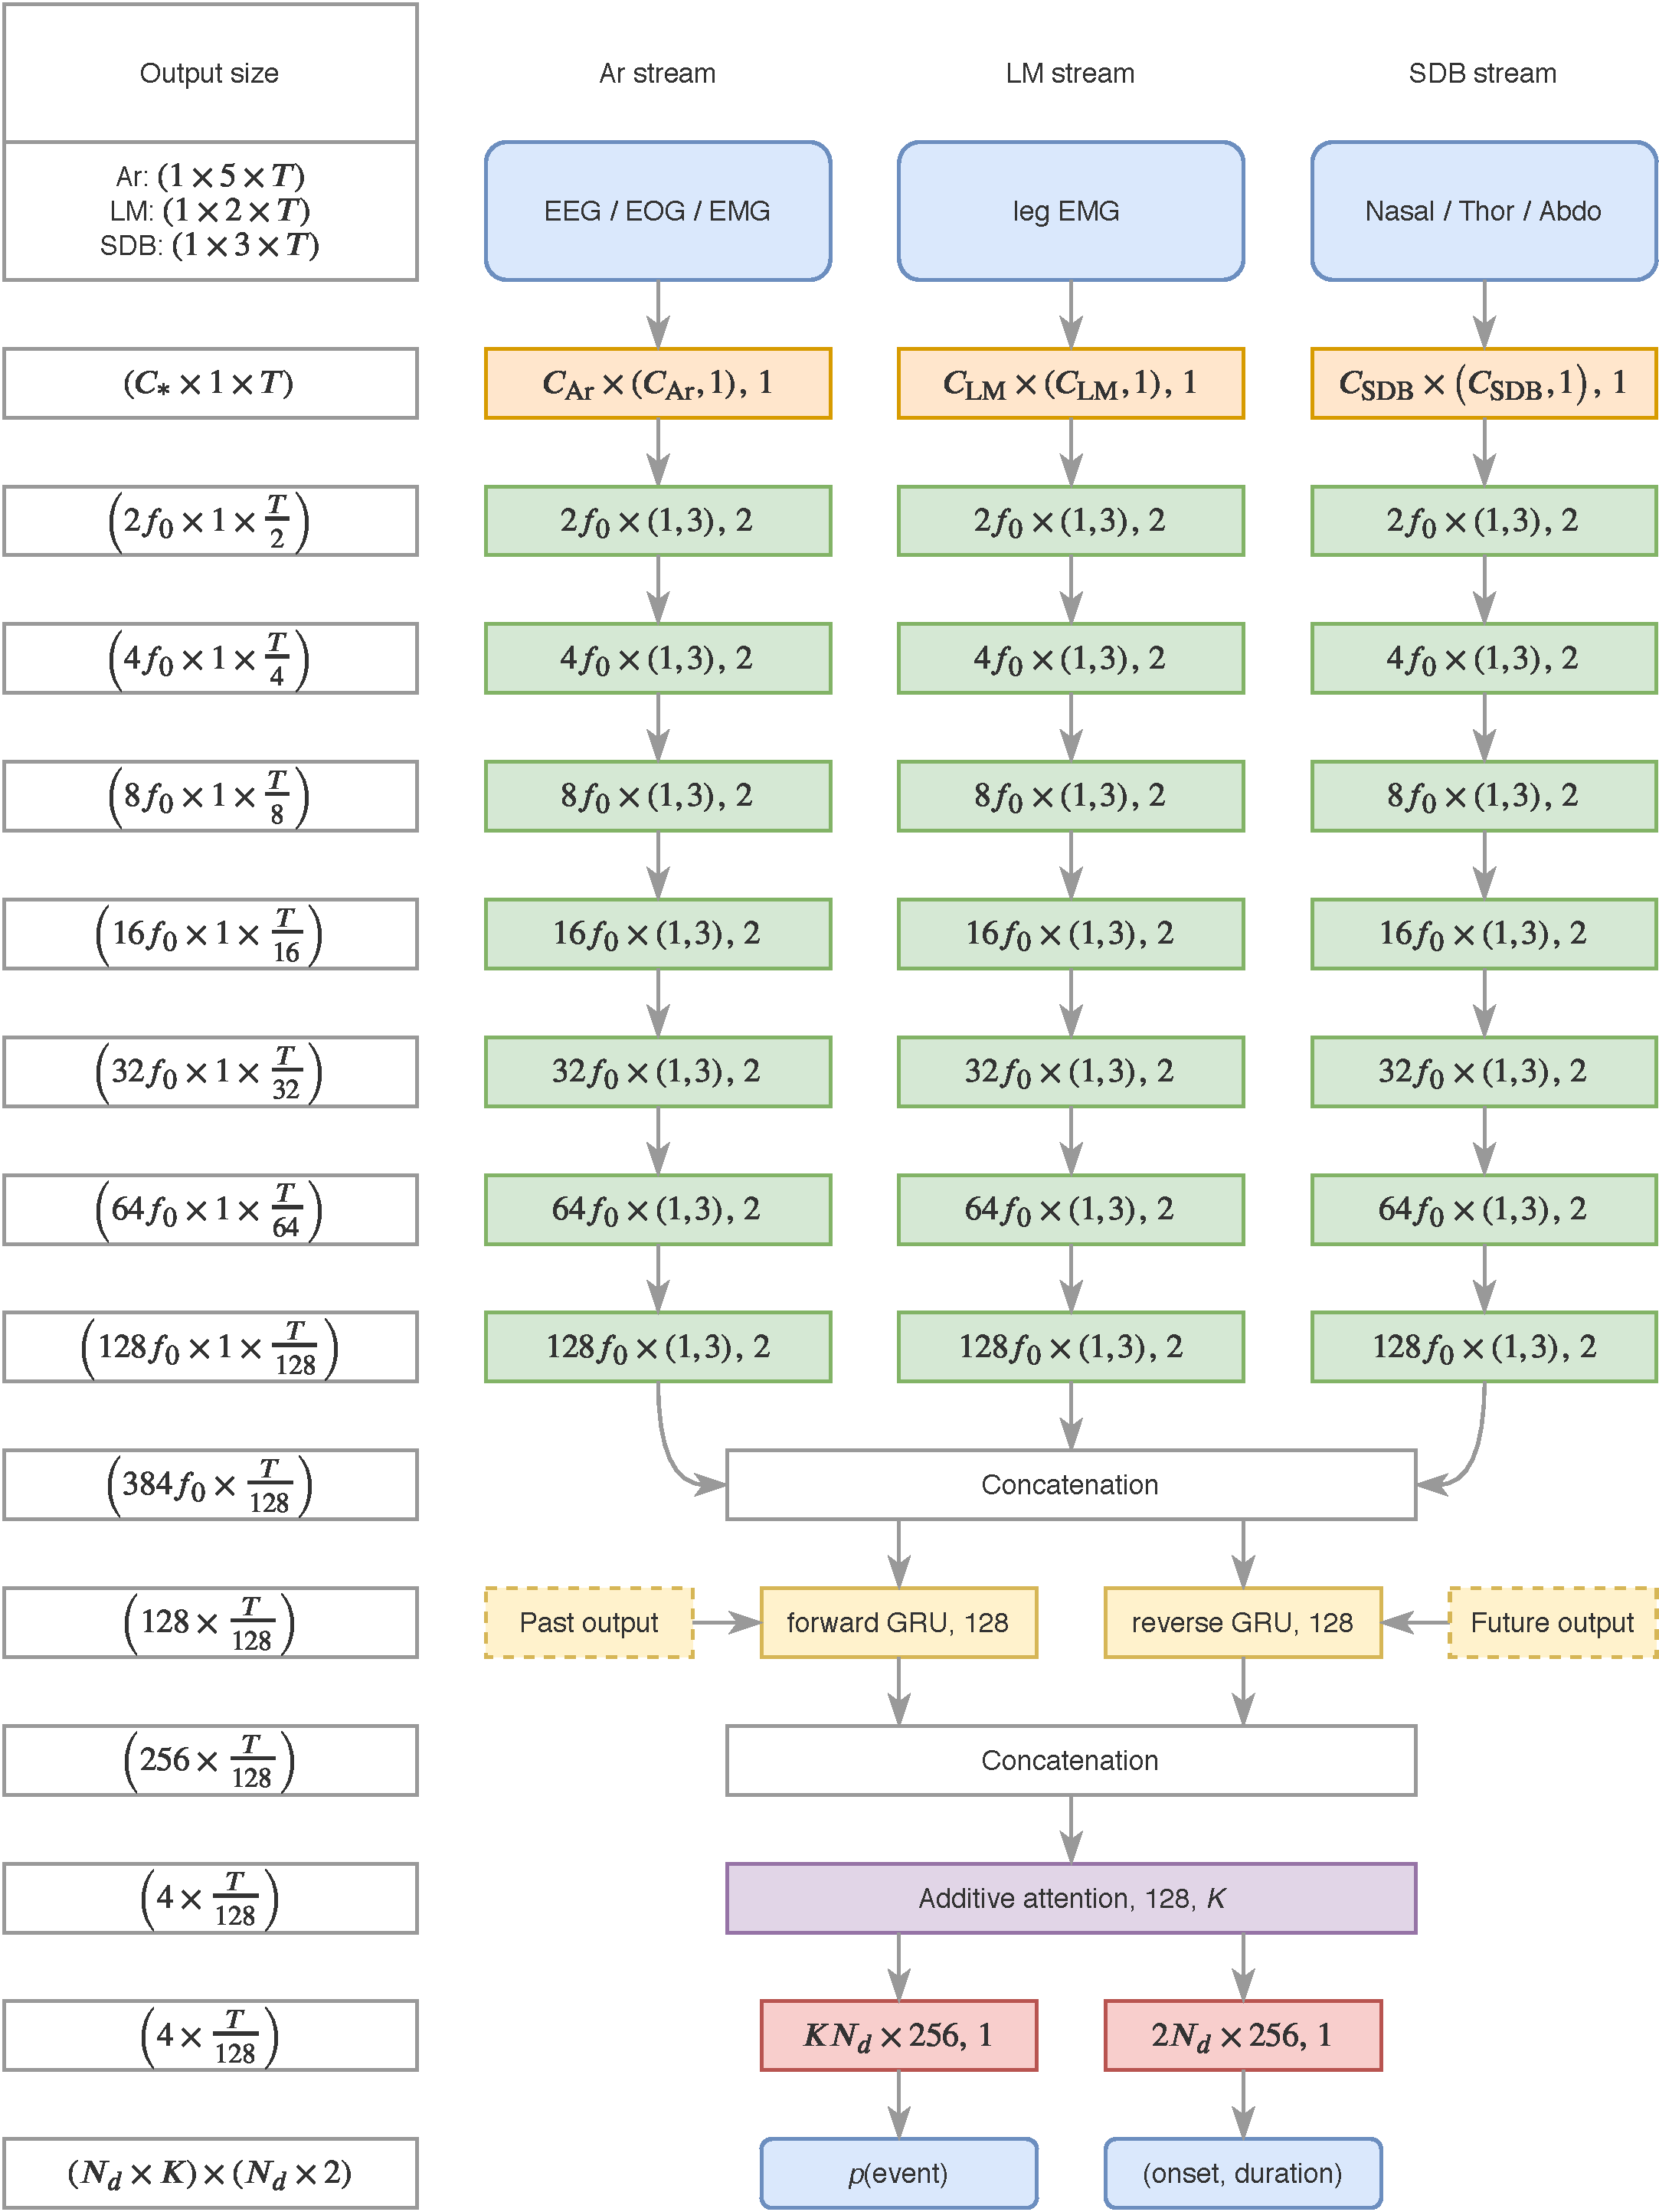
\includegraphics[width=\linewidth]{figures/paper-vi/msed_architecture.pdf}
    \caption[\acs{MSED} network architecture]{\acs{MSED} network architecture. The left column shows the output dimensions for each operation as (number of filters[ x singleton] x time steps). Each stream on the right (green) processes a separate set of input channels (blue, top), the results of which are concatenated before the \ac{bGRU} (yellow). The outputs from the additive attention layer (purple) are convolved in the final classification and localization layers (red) to output the probabilities for each event class, and the predicted onset and duration of each event (blue, bottom). Convolution layers (orange, green, red) are detailed as [number of feature maps x kernel size, stride]. Recurrent layer (yellow) shows the direction and number of hidden units. Additive attention layer (purple) is described with the number of hidden and output units.}
    \label{fig:event-detection:paper-vi:architecture}
    \end{adjustwidth*}
\end{figure}

\subsubsection{Stream specifics}
Each stream is comprised of two components.
First, a mixing module \( \varphi_\text{mix} : \R{C_{\ast} \times T} \rightarrow \R{C_{\ast} \times T} \) computes a non-linear mixing of the \(C\) channels using a set of \(C\) single-strided 1-dimensional filters \(\mathbf{w} \in \R{C \times C}\) and \ac{ReLU} activation~\cite{Nair2010}, such that \(\func{\varphi_\text{mix}}{\mathbf{x}} = \max \braces*{0, \mathbf{w} \otimes \mathbf{x} + \mathbf{b}}\), where the \(\max\) operation introduces the non-linearity, \(\otimes\) is the conv operator over the \(C\) feature maps, and \(\mathbf{b}\in \R{C}\) is a bias vector (in this case \(\mathbf{b} = 0\)).
Second, the output activations from \(\varphi_\text{mix}\) are used as input to a deep neural network module \(\varphi_\text{feat} : \R{C_\ast \times T} \rightarrow \R{f^{\prime} \times T^{\prime}}\), which transforms the input feature maps to a \(f^{\prime} \times T^{\prime}\) feature space with a temporal dimension reduced by a factor of \(\frac{T}{T^{\prime}}\).
The feature extraction module \(\varphi_\text{feat}\) is realized using \(k_\text{max}\) successive conv operations with an increasing number of filters \(f^{\prime} = f_0 2^{k-1}, \, k \in \llbracket k_\text{max} \rrbracket\), where \(f_0\) is a tunable base filter number.
Each conv feature map is normalized using \ac{BN}~\cite{Ioffe2015}, such that if \(\mathbf{\tilde{z}} \in \R{f^{\prime} \times T^{\prime}}\) denotes the output from a conv operation, the subsequent normalized version is computed as
\begin{equation}
    \mathbf{z} = \boldsymbol{\gamma}\frac{\mathbf{\tilde{z}} - \expect{\mathbf{\tilde{z}}}}{ \sqrt{\variance{\mathbf{\tilde{z}}} + \epsilon}} + \boldsymbol{\beta},
\end{equation}
where \(\expect{\mathbf{\tilde{z}}} \in \R{f^{\prime}}, \, \variance{\mathbf{\tilde{z}}} \in \R{f^{\prime}}_+\) is the expectation and variance over the temporal dimension of each feature map, \(\epsilon\) is a small constant, and \(\braces*{\boldsymbol{\gamma}, \, \boldsymbol{\beta}} \in \R{f^{\prime}} \times \R{f^{\prime}}\) are learnable parameters representing the mean and bias for each feature map.
Each normalized conv output is subsequently activated using \ac{ReLU}.

\subsubsection{Feature fusion for sequential processing}
The outputs from the three feature extraction streams are subsequently fused by concenating each output vector \( \mathbf{z}_{\ast} \) into a combined feature vector \(\mathbf{z}=\parentheses*{\mathbf{z}_\text{ar}, \mathbf{z}_\text{lm}, \mathbf{z}_\text{sdb}} \in \R{3f^{\prime} \times T^{\prime}}\).
We introduce sequential modeling of the feature vectors using a \ac{bGRU}~\cite{Cho2014}, which has the advantage over other \ac{RNN}-based models such as the \ac{LSTM} of having fewer trainable parameters while still being powerful enough to model complex, temporal relationships~\cite{Chung2014}.
The output of the \ac{GRU} for timestep \textit{t} is a vector \( \mathbf{h}_{t} = \parentheses*{{\mathbf{h}_{t}^{\mathsf{f}}}, {\mathbf{h}_{t}^{\mathsf{b}}}} \in \R{2n_h}\) containing the concatenated outputs from the forward (\textsf{f}) and backward (\textsf{b}) directions.
Each directional feature vector is calculated as a weighted combination of a gated new input \(\mathbf{n}_t\) and the feature vector from the previous timestep \(\mathbf{h}_{t-1}\)
\begin{equation}
    \mathbf{h}^{\ast}_t = \parentheses*{1 - \mathbf{u}_t} \otimes \mathbf{n}_t + \mathbf{u}_t \otimes \mathbf{h}_{t-1}.
\end{equation}
The update gate \(\mathbf{u}_t\) and gated new input \(\mathbf{n}_t\) are computed as
\begin{align}
    \mathbf{u}_t &= \func{\sigma}{\mathbf{W}_{u}^z \mathbf{z}_t + \mathbf{b}_u^z + \mathbf{W}_{u}^h \mathbf{h}_{t-1} + \mathbf{b}_u^h}, \\
    \mathbf{n}_t &= \func{\tanh}{\mathbf{W}_{n}^z \mathbf{z}_t + \mathbf{b}_n^z + \mathbf{r}_t \otimes \parentheses*{ \mathbf{W}_{n}^h \mathbf{h}_{t-1} + \mathbf{b}_n^h }},
\end{align}
where \(\mathbf{W}^\ast_\ast, \mathbf{b}^\ast_\ast\) are weight matrices and bias vectors, respectively, and \(\mathbf{r}_t\) is a reset gate computed as
\begin{equation}
    \mathbf{r}_t = \func{\sigma}{\mathbf{W}_r^z \mathbf{z}_t + \mathbf{b}_r^z + \mathbf{W}_h^r \mathbf{h}_{t-1} + \mathbf{b}_h^r}.
\end{equation}

\subsubsection{Additive attention}
The attention mechanism is a powerful technique to introduce a way for the network to focus on relevant regions and disregard irrelevant regions of a data sample, and is a key part of the highly successful Transformer model~\cite{Vaswani2017} and the subsequent state-of-the-art BERT model for natural language processing~\cite{Devlin2019}.
In this work, we implemented a simple, but powerful, \textit{additive attention} mechanism~\cite{Bahdanau2015}, which computes \textit{context}-vectors \(\mathbf{c} \in \R{2n_h}\) for each event class as the weighted sum of the feature vector outputs \(\mathbf{h}\in\R{2n_h \times T^{\prime}}\) from the \(\varphi_h\).
Formally, attention is computed as
\begin{equation}
    \mathbf{c} = \mathbf{h}\cdot\boldsymbol{\alpha} = \sum_{t=1}^{T^{\prime}} \mathbf{h}_t \boldsymbol{\alpha}_t,
\end{equation}
where \(T^{\prime}\) is the reduced temporal dimension, \(\mathbf{h}_t\) is the feature vector for time step \(t\), and \(\boldsymbol{\alpha}_t \in \R{K}\) is the attention weight computed as
\begin{equation}
    \boldsymbol{\alpha}_t = \frac{ \func{\exp}{\func{\tanh}{\mathbf{h}_t\mathbf{W}_\text{u}}\mathbf{W}_{a}}}{\sum_{\tau}^{T^{\prime}}\func{\exp}{\func{\tanh}{\mathbf{h}_\tau\mathbf{W}_\text{u}}\mathbf{W}_{a}}}.
\end{equation}
Here, \(\mathbf{W}_u \in \R{2n_h \times n_a}\) and \(\mathbf{W}_a \in \R{n_a \times K}\) are linear mappings of the feature vectors, and \(\tanh\) is the hyperbolic tangent function.

\subsubsection{Detection}
The final event classification and localization is handled by two modules, \(\psi_{\mathrm{clf}} : \R{2n_h \times K} \to \R{N_d \times K}\) and \( \psi_{\mathrm{loc}} : \R{2n_h \times K} \to \R{N_d \times 2} \), respectively.
The classification module \(\psi_\text{clf} : \mathbf{c} \mapsto \mathbf{p}\) outputs a tensor \(\mathbf{p} \in \brackets*{0, 1}^{N_d \times K}_{+} \) containing predicted event class probabilities for each default event window.
The localization module \(\psi_\text{loc} : \mathbf{c} \mapsto \mathbf{y}\) outputs a tensor \(\mathbf{y} \in \R{N_d \times 2}\) containing encoded relative onsets and durations for a detected event for each default event window.
% The output from $\varphi_{\mathrm{att}}$ is processed by two separate blocks: $ \psi_{\mathrm{clf}} : \R{f^{\prime} \times 2 \times T^{\prime}} \to \R{\left( K + 1 \right) \! N_d \times 1 \times T^{\prime}} $ outputs the tensor $\mathbf{p}$ containing predicted arousal probabilities for each time point $t \in \llbracket T^{\prime} \rrbracket$ for each default event window.
% $ \psi_{\mathrm{loc}} : \R{f^{\prime} \times 2 \times T^{\prime}} \to \R{2N_d \times T^{\prime}} $ outputs the tensor $\mathbf{y}$ containing predicted start time and durations of arousal events.
% Both $\psi_{\mathrm{clf}}$ and $\psi_{\mathrm{loc}}$ are implemented using $\left(2, 1\right)$ convolutions rather than convolutions over the entire volume as in~\cite{Chambon2018b, Chambon2019, Olesen2019}.
% This serves a dual purpose: the first is to reduce the number of parameters to make the network more memory-efficient, while the second purpose is to allow the kernel and feature maps to be temporally invariant.

\subsubsection{Loss function}
Similar to~\cite{Olesen2020DeepDetection}, we optimized the network parameters according to a three-component loss function consisting of 
\begin{enumerate*}[before=\unskip{: }, itemjoin={{; }}, itemjoin*={{, and }}, label=\roman*)]
\item a localization loss \( \ell_{\mathrm{loc}} \)
\item a positive classification loss $\ell_{+}$
\item a negative classification loss $\ell_{-}$
\end{enumerate*}, 
such that the total loss $\ell$ was defined by
\begin{equation}\label{eq:loss}
    \ell = \ell_{\mathrm{loc}} + \ell_{+} + \ell_{-}.
\end{equation}
The localization loss $\ell_{\mathrm{loc}}$ was calculated using a Huber function
\begin{equation}
    \ell_{\mathrm{loc}} = \frac{1}{N_{+}} \, \sum_{\mathclap{i \in \pi_{+}}}\!{f_{H}^{(i)}} \\
    % \ell_{\mathrm{loc}} = \frac{1}{\sum_{i}{i \\pi \backslash \emptyset}} \sum_{i \in \pi \backslash \emptyset}\!{h^{(i)}} \\
\end{equation} 
\begin{equation}
    \mathbf{f}_{H} =
    \begin{cases}
        0.5 \parentheses*{ \mathbf{y} - \mathbf{t} }^2, & \text{if } \abs*{ \mathbf{y} - \mathbf{t} } < 1, \\
        \abs*{ \mathbf{y} - \mathbf{t} } - 0.5, & \text{otherwise,}
    \end{cases}
\end{equation}
where $i \in \pi_{+}$ yields indices of event windows with positive targets, \ie event windows matched to an arousal, \ac{LM} or \ac{SDB} target, and $N_{+}$ is the number of positive targets in the given data segment.

The positive classification loss component $\ell_{+}$ was calculated using a simple cross-entropy over the event windows matched to an arousal, \ac{LM}, or \ac{SDB} event:
\begin{equation}
    \ell_{+} = \frac{1}{N_{+}} \, \sum_{i \in \pi_{+}} \sum_{k \in \llbracket K \rrbracket} \pi^{(i)}_{k} \log p^{(i)}_{k}, \quad \text{where} \quad p^{(i)}_{k} = \frac{\exp{s^{(i)}_{k}}}{\sum_{j} \exp s^{(i)}_{j}},
\end{equation}
and $\pi^{(i)}_k$, $p^{(i)}_k$, and $s^{(i)}_k$ are the true class probability, predicted class probability, and logit score for the \textit{i}th event window containing a positive sample.

Similar to~\cite{Chambon2018b, Chambon2019}, the negative classification loss $\ell_{-}$ was calculated using a hard negative mining approach to balance the number of positive and negative samples in a data segment after matching default event windows to true events~\cite{Liu2016}.
Specifically, this is accomplished by calculating the probability for the negative class (no event) for each unmatched default event window, and then calculating the cross entropy loss using the \textit{Z} most probable samples.
In our experiments, we set the ratio of positive to negative samples as 1:3, such that the calculation of $\ell$ involves $Z=3$ times as many negative as positive samples.

We also explored a focal loss objective function for computing $\ell_{+}$ and $\ell_{-}$~\cite{Lin2020}, however, we found that this approach severely deteriorated the ability of the network to accurately detect \ac{LM} and \ac{SDB} events compared to using worst negative mining.
% \begin{align}
%     \ell_{+} &= \frac{1}{N_{\pi \backslash \emptyset}} \sum_{i \in \pi \backslash \emptyset}\!{-\alpha \left( 1 - \mathbf{p} \right)^{\gamma}\log \left( \mathbf{p} \right)}, \, \text{and} \\
%     \ell_{-} &= \frac{1}{N_{\pi = \emptyset}} \sum_{i \in \pi = \emptyset}\!{-\alpha \left( 1 - \mathbf{p} \right)^{\gamma}\log \left( \mathbf{p} \right)},
% \end{align}
% where $\alpha=0.25$ and $\gamma=2$.
% This serves to counter the class imbalance in a single data segment, which typically consists of many event windows with few positive examples.

\subsubsection{Optimization}
The network parameters were optimized using adaptive moment estimation (Adam) according to the loss function described in~\cref{eq:loss}~\cite{Kingma2015}.
This algorithms uses first ($m$) and second ($v$) moment estimations of gradients to update the model parameters $\theta$ of a differentiable function $f$ at time $t$:
\begin{align}
    m^{(t)} &= \beta_1 m^{(t-1)} + \parentheses*{ 1 - \beta_1 } \func{\nabla_\theta f^{(t)}}{\theta^{(t-1)}} \\
    v^{(t)} &= \beta_2 v^{(t-1)} + \parentheses*{ 1 - \beta_2 } \func{\nabla^2_\theta f^{(t)}}{\theta^{(t-1)}},
\end{align}
where $\beta_1, \beta_2$ are exponential decay rates for the first and second moment, respectively, $\nabla$ is the gradient vector with respect to $\theta$, and $\nabla^2_\theta$ is the Hadamard product \(\nabla_\theta f \odot \nabla_\theta f\).
The moment vectors are initialized with \(0\)'s, which induce a bias towards zero.
This can be offset by computing a bias-corrected estimate of each moment vector as
\begin{align}
    \hat{m}^{(t)} &= \frac{m^{(t)}}{1 - \beta^t_1} \\
    \hat{v}^{(t)} &= \frac{v^{(t)}}{1 - \beta^t_2},
\end{align}
which yields the final update to \(\theta\) as
\begin{equation}
    \theta^{(t)} = \theta^{(t-1)} - \eta \frac{\hat{m}^{(t)}}{\sqrt{\hat{v}^{(t)}} + \epsilon},
\end{equation}
where \(\eta\) is the learning rate.

\subsubsection{Experimental setups}
In our experiments, we fixed the exponential decay rates at \((\beta_1, \beta_2) = (0.9, 0.999)\), the learning rate at \(\eta = 10^{-3}\), and \(\epsilon = 10^{-8}\).
The learning rate was decayed in a step-wise manner by multiplying \( \eta \) with a factor of 0.1 after 3 consecutive epochs with no improvement in loss value on the validation dataset.

Similarly, we employed an early stopping scheme by monitoring the loss on the validation dataset and stopping the model training after 10 epochs of no improvement on \(\mathcal{D}_\textsc{eval}\).

We tested four types of models in two categories: the first is a default split-stream model as shown in~\cref{fig:event-detection:paper-vi:architecture} with and without weight decay (splitstream, splitstream-wd).
The second is a variation of the split-stream model, but where the \(\psi_\text{clf}\) and \(\psi_\text{loc}\) modules are realized using depth-wise convolutions, such that each attention group is used only for that type of event.
The second category is also tested with and without weight decay (splitstream-dw, splitstream-dw-wd).


\subsubsection{Performance evaluation}
Performance was quantified using precision, recall and F1 scores.
Statistical significance in F1 score between groups was assessed with Kruskall-Wallis \textit{H}-tests.
The performance of joint vs. single-event detection models was tested with Wilcoxon signed rank tests for matched samples.
The relationships between true and predicted \ac{ArI}, \ac{AHI}, and \ac{LMI} were assessed using linear models and Pearsons \(r^2\).
Significance was set at \(\alpha=0.05\).

\subsection{Results and discussion}
\subsubsection{Model architecture evaluation}

\begin{figure}[tb]
    \centering
    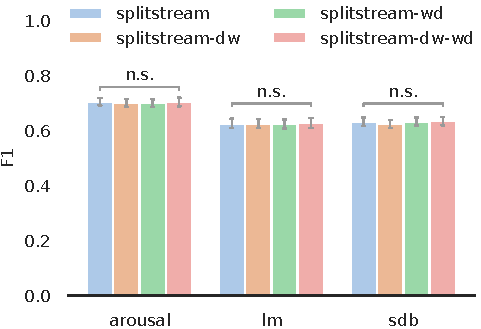
\includegraphics[width=0.75\linewidth]{figures/paper-vi/model_types (2).pdf}
    \caption[Architecture optimization]{Architecture optimization.}\label{fig:my_label}
\end{figure}

We found no significant differences in F1 performance for either \ac{Ar} (Kruskal-Wallis \(H = 0.961, \, p = 0.811\)), \ac{LM} (\( H = 0.230, \, p = 0.973 \)), or \ac{SDB} detection (\( H = 2.838, \, p = 0.417 \)), when evaluating the model architectures on \(\mathcal{D}_\textsc{eval}\).
Based on this result, all further modeling was based on the default splitstream architecture for simplicity.


\subsubsection{Joint vs. single event detection}

For each event type, we evaluated the F1 score as a function of classification threshold \(\theta\) on \(\mathcal{D}_\textsc{eval}\) for both the joint detection model as well as the single-event models.
It can be observed in~\cref{fig:f1_theta_eval} that for all three events, the joint detection model achieves higher F1 score, although the apparent increase is not as large for \ac{LM} detection.
This was also observed when evaluating the joint and single detection models with optimized thresholds on \(\mathcal{D}_\textsc{test}\) for both \ac{Ar} (Wilcoxon \(W = 30440.0, \, p = \num{2.481e-127}\)), \ac{LM} (\(W = 101103.0, \, p = \num{6.454e-60}\)), and \ac{SDB} detection (\(W = 93647.0, \, p = \num{2.378e-64}\)). Precision, recall and F1 scores for optimized models evaluated on \(\mathcal{D}_\textsc{test}\) are shown in~\cref{tab:test_performance}.
These findings are interesting, because they provide evidence that the presence of different event types can module the detection of others, and that this can be modeled using automatic methods.
This is in line with what previous studies have found \eg on event-by-event scoring agreement in arousals, which improved significantly from \SIrange{0.59}{0.91}{\percent}, when including respiratory signals in the analysis~\cite{Thomas2003}.

\begin{figure}[tb]
    \centering
    \begin{adjustwidth*}{}{-\marginparwidth-\marginparsep}
    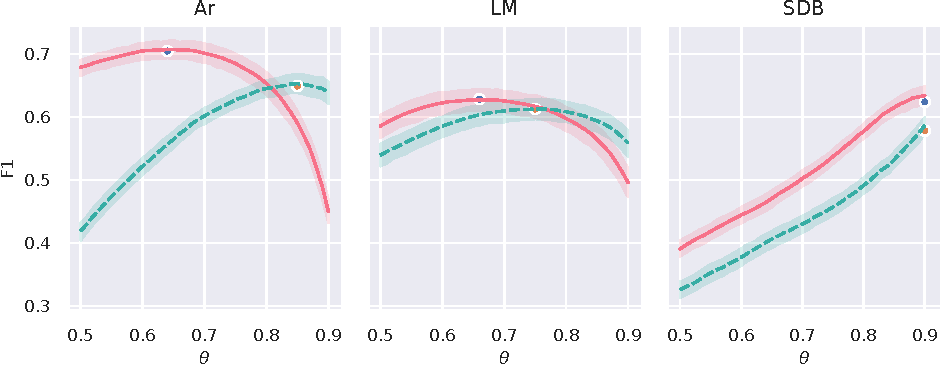
\includegraphics[width=\linewidth]{figures/paper-vi/f1_threshold (1).pdf}
    \caption[Optimizing F1 performance]{Optimizing F1 performance on \(\mathcal{D}_\textsc{eval}\) as a function of \(\theta\)). Full lines correspond to the joint model and dashed lines are the corresponding single-event detection model. The blue and orange dots correspond to optimized model performance on \(\mathcal{D}_\textsc{test}\).}
    \label{fig:f1_theta_eval}
    \end{adjustwidth*}
\end{figure}

\begin{figure}[tb]
    \centering
    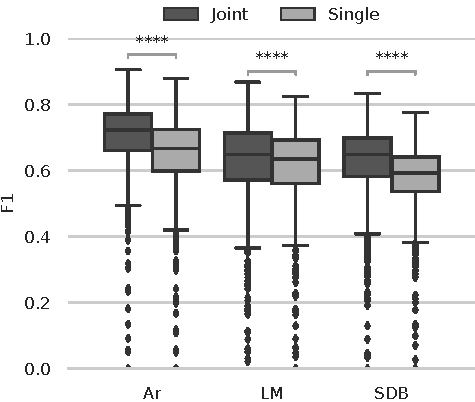
\includegraphics[width=0.75\linewidth]{figures/paper-vi/f1_dist_boxplot.pdf}
    \caption[Optimized join and single-event model performance]{Evaluating optimized joint and single-event detection models on \(\mathcal{D}_\textsc{test}\). \(^{****}\): \(p < \num{10e-4}\). %
    \describe{Ar}; %
    \describe{LM}; %
    \describe{SDB}.}
    \label{fig:f1_test}
\end{figure}

% \plusminus{1}{4}
\begin{table}[tb]
\small
    \centering
    % \renewcommand*{\arraystretch}{1.2}
    \begin{threeparttable}
    \caption[Performance scores for optimized models on \(\mathcal{D}_\textsc{test}\)]{Performance scores for optimized models evaluated on \(\mathcal{D}_\textsc{test}\).}
    \label{tab:test_performance}
    \begin{tabular}{@{}llccc@{}}
        \toprule
        \textbf{Event} & \textbf{Model} & \textbf{Precision} & \textbf{Recall} & \textbf{F1} \\
        \midrule
        \ac{Ar}  & Joint  & \plusminus{0.759}{0.114} & \plusminus{0.672}{0.125} & \plusminus{0.704}{0.106} \\
                 & Single & \plusminus{0.777}{0.107} & \plusminus{0.571}{0.127}	 & \plusminus{0.649}{0.113} \\
        \ac{LM}  & Joint  & \plusminus{0.650}{0.169} & \plusminus{0.647}{0.120}	& \plusminus{0.628}{0.123} \\
                 & Single & \plusminus{0.661}{0.166} & \plusminus{0.607}{0.116} & \plusminus{0.613}{0.116} \\
        \ac{SDB} & Joint  & \plusminus{0.817}{0.142} & \plusminus{0.526}{0.146} & \plusminus{0.624}{0.115} \\
                 & Single & \plusminus{0.765}{0.142} & \plusminus{0.486}{0.121} & \plusminus{0.578}{0.097} \\
        \bottomrule
    \end{tabular}
    \begin{tablenotes}
    \item Metrics are shown aggregated across \acp{PSG}. %
    \describe{Ar}; %
    \describe{LM}; %
    \describe{SDB}.
    \end{tablenotes}
    \end{threeparttable}
\end{table}

% \begin{tabular}

% \end{tabular}

\subsubsection{Detection vs. manual scorings}

For each event type, we computed the correlation coefficient between the predicted and true index values (arousal index, ArI; apnea-hypopnea index, AHI; limb movement index, LMI), which is shown in~\cref{fig:event-detection:paper-vi:correlation_plot}.
We found a large positive correlation between true and predicted values for \ac{ArI} (\(r^2=0.73\), \(p=\num{2.5e-285}\)), \ac{AHI} (\(r^2=0.77\), \(p=\num{9.3e-316}\)), and \ac{LMI} (\(r^2=0.78\), \(p=\num{3.1e-321}\)).

A similar study using an automatic method for automatic detection of \ac{SDB}\graffito{The authors pooled obstructive, central, mixed apneas, and 4\% hypopneas into one category, \emph{apnea}.} and \ac{LM} events found similar or higher correlations between automatic and manual scorings (\(r^2 = 0.85\), and \(r^2 = 0.79\), respectively), although their findings were based on almost 5 times as much data~\cite{Biswal2018}.

\begin{figure}
    % \centering
    \begin{adjustwidth*}{}{-\marginparwidth-\marginparsep}
    \myfloatalign   
    \subfloat[]
    {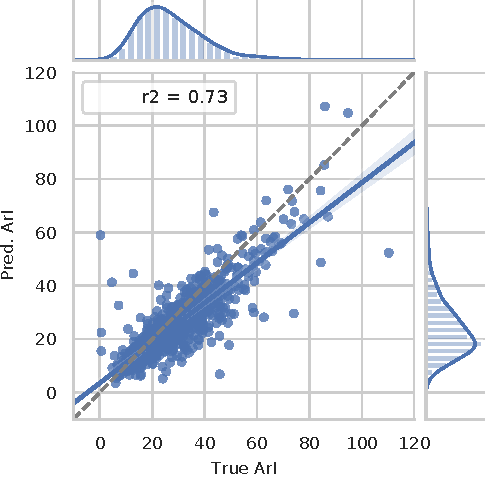
\includegraphics[width=0.5\linewidth]{figures/paper-vi/linearplot_ari.pdf}\label{fig:event-detection:paper-vi:ari}}
    \subfloat[]
    {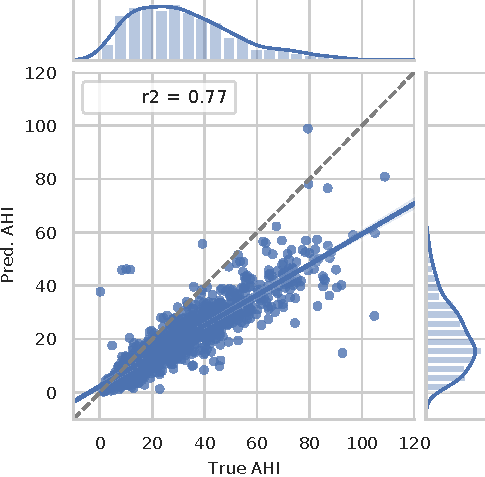
\includegraphics[width=0.5\linewidth]{figures/paper-vi/linearplot_ahi.pdf}\label{fig:event-detection:paper-vi:ahi}}\\
    \subfloat[]
    {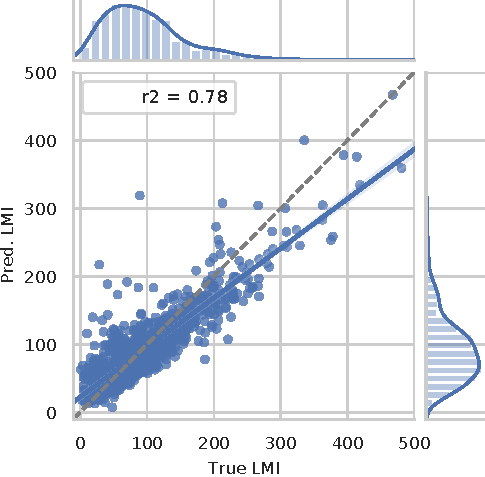
\includegraphics[width=0.5\linewidth]{figures/paper-vi/linearplot_lmi.pdf}\label{fig:event-detection:paper-vi:lmi}}
    \caption[Correlation between true and predicted indices]{Pearson correlation plots for each event type index between true and predicted values. The linear relationship is indicated with solid blue with 95\% confidence intervals in light blue.
    Grey dashed lines indicate perfect correlation lines.
    \describe{ArI}; %
    \describe{AHI}; %
    \describe{LMI}.}
    \label{fig:event-detection:paper-vi:correlation_plot}
    \end{adjustwidth*}
\end{figure}


\subsubsection{Temporal characteristics}
We compared the temporal precision between manual and automatic event scoring by looking at the errors in onset (\(\Delta\text{onset}\)), offsets (\(\Delta\text{offset}\)), and durations (\(\Delta\text{dur.}\)) calculated as
\begin{align}
    \Delta\,\text{onset} &= \text{onset}_{\text{automatic}} - \text{onset}_{\text{manual}} \\
    \Delta\,\text{offset} &= \text{offset}_{\text{automatic}} - \text{offset}_{\text{manual}} \\
    \Delta\,\text{dur} &= \text{dur}_{\text{automatic}} - \text{dur}_{\text{manual}}
\end{align}
so that positive values of \(\Delta\,\text{onset}, \Delta\,\text{offset}\) corresponds to a positive shift to the right (delayed prediction), and positive values of \(\Delta\,\text{dur.}\) meaning an overestimation of the event duration compared to manual scoring.
This is shown in~\cref{fig:event-detection:paper-vi:temporal-morphology}, where the blue distributions are the joint detection model for each event type, and the orange distributions are the corresponding single-event models. 
The distributions are shown as kernel density estimates superimposed on a histogram.
For \ac{Ar} events, the model overestimates the duration on average by a couple of seconds, which is caused by an earlier prediction of onset and delayed prediction of termination.
For \ac{LM} events, the model underestimates the duration by about half a second on average, which is due to earlier prediction of termination.
For \ac{SDB} events, the model overestimates the duration by about 25 seconds on average, which is caused by an earlier prediction of onset and delayed prediction of termination.
These errors in predicted durations reflects the temporal characteristics of these events; \acp{LM} are shorter events\graffito{Between \SIrange{0.5}{10}{\second} per definition.}, and it is thus unlikely to be overestimated by several seconds, while \acp{SDB} are longer events by one to two orders of magnitude, which also increases the size of the errors. 
\acp{Ar} events are intermediate in length compared to \acp{LM} and \acp{SDB}, which is reflected in the error distributions.
\begin{figure}[tb]
    \centering
    \begin{adjustwidth*}{}{-\marginparwidth-\marginparsep}
    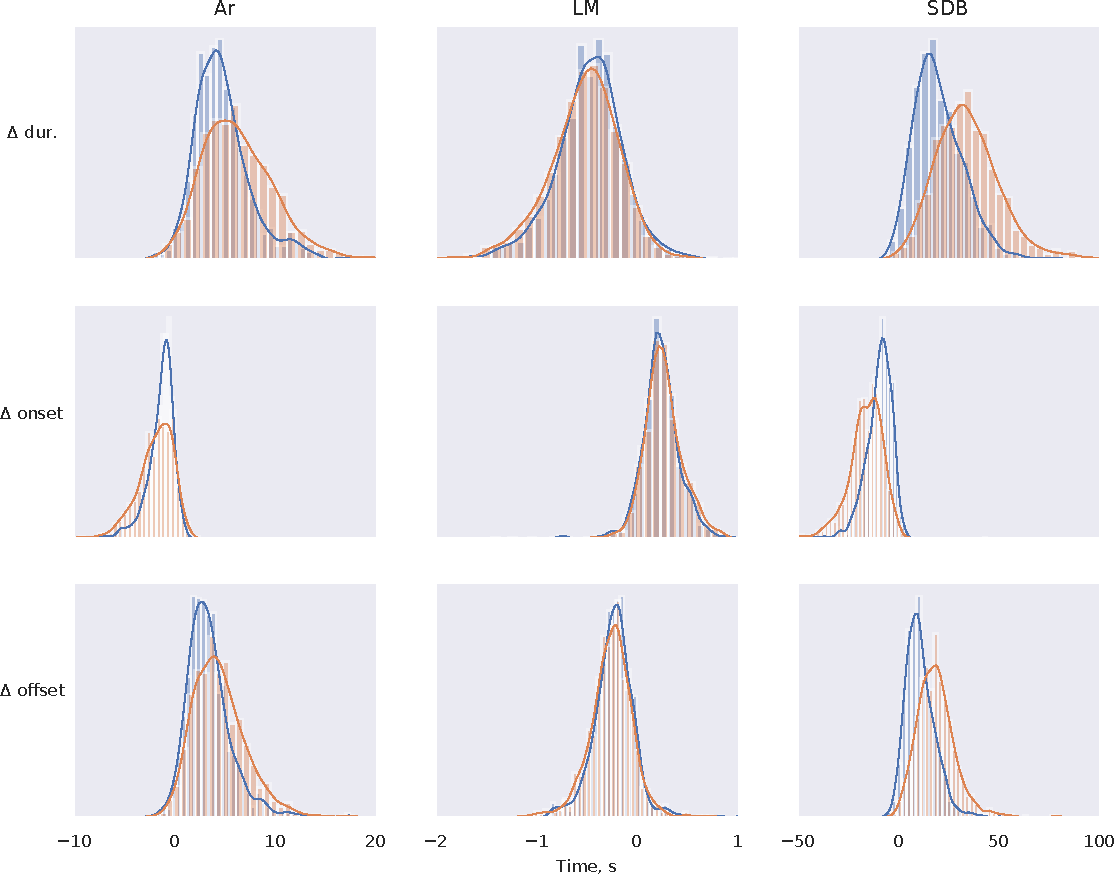
\includegraphics[width=\linewidth]{figures/paper-vi/distribution_plots.pdf}
    \caption[Distribution of temporal error metrics]{Temporal error metrics distributions across all events and \acp{PSG}. Positive values of \(\Delta\text{onset}, \Delta\text{offset}\) means delayed predictions, while positive values of \(\Delta\text{dur.}\) means to an overestimation of event duration. Blue distributions are joint detection models, while orange distributions are the corresponding single-event models. Distributions are shown as kernel density estimates superimposed on a histogram. %
    \describe{Ar}; %
    \describe{LM}; %
    \describe{SDB}.}
    \label{fig:event-detection:paper-vi:temporal-morphology}
    \end{adjustwidth*}
\end{figure}


% \subsection{Discussion}
% Discussion points:
% \begin{itemize}
%     \item We found that jointly predicting events improved detection performance across the board. Similarly, \citeauthor{Thomas2003} found that event-by-event scoring agreement in scoring arousals improved significantly from \SIrange{0.59}{0.91}{\percent}, when including respiratory signals in the analysis~\cite{Thomas2003}.
% \end{itemize}